\documentclass{beamer}
%%%%%%%%%%%%%%%%%%%%%%%%%%%%%%%%%%%%%%%%%%%%%%%%%%%%%%%%%%%%%%%%%%%%%%%%%%%%%%%%%%%%%%%%%%%%%%%%%%
\setbeamertemplate{navigation symbols}{}
\usepackage{beamerthemeshadow}
\usefonttheme{serif}
%%%%%%%%%%%%%%%%%%%%%%%%%%%%%%%%%%%%%%%%%%%%%%%%%%%%%%%%%%%%%%%%%%%%%%%%%%%%%%%%%%%%%%%%%%%%%%%%%%
\usepackage{graphicx}
\graphicspath{ {res/} }
%%%%%%%%%%%%%%%%%%%%%%%%%%%%%%%%%%%%%%%%%%%%%%%%%%%%%%%%%%%%%%%%%%%%%%%%%%%%%%%%%%%%%%%%%%%%%%%%%%
\usepackage{polyglossia}
\setdefaultlanguage{armenian}
\setotherlanguages{english}
\usepackage{fontspec}
\newfontfamily\armenianfont{DejaVu Sans}
%%%%%%%%%%%%%%%%%%%%%%%%%%%%%%%%%%%%%%%%%%%%%%%%%%%%%%%%%%%%%%%%%%%%%%%%%%%%%%%%%%%%%%%%%%%%%%%%%%
\usepackage{minted}
\setminted[cpp]{fontsize=\footnotesize}
\setmonofont{Consolas}
%%%%%%%%%%%%%%%%%%%%%%%%%%%%%%%%%%%%%%%%%%%%%%%%%%%%%%%%%%%%%%%%%%%%%%%%%%%%%%%%%%%%%%%%%%%%%%%%%%
\usepackage{xltxtra}
\usepackage{hyperref}
%%%%%%%%%%%%%%%%%%%%%%%%%%%%%%%%%%%%%%%%%%%%%%%%%%%%%%%%%%%%%%%%%%%%%%%%%%%%%%%%%%%%%%%%%%%%%%%%%%
\usetheme{Luebeck}
\usecolortheme{crane}
%%%%%%%%%%%%%%%%%%%%%%%%%%%%%%%%%%%%%%%%%%%%%%%%%%%%%%%%%%%%%%%%%%%%%%%%%%%%%%%%%%%%%%%%%%%%%%%%%%
\definecolor{HTDark}{rgb}{0.04706, 0.13725, 0.26667} % primary color
\definecolor{HTLight}{rgb}{0.3686, 0.5255, 0.6235}   % secondary color
\setbeamercolor{palette primary}{bg=HTDark,fg=white}
\setbeamercolor{palette secondary}{bg=HTDark,fg=white}
\setbeamercolor{palette tertiary}{bg=HTDark,fg=white}
\setbeamercolor{palette quaternary}{bg=HTDark,fg=white}
\setbeamercolor{structure}{fg=HTDark} % itemize, enumerate, etc
\setbeamercolor{section in toc}{fg=HTDark} % TOC sections
\setbeamercolor{block title}{fg=white,bg=HTDark}
\setbeamercolor{block body}{fg=white, bg=HTLight}
\setbeamercolor{subsection in head/foot}{bg=HTLight,fg=white}
%%%%%%%%%%%%%%%%%%%%%%%%%%%%%%%%%%%%%%%%%%%%%%%%%%%%%%%%%%%%%%%%%%%%%%%%%%%%%%%%%%%%%%%%%%%%%%%%%%


\begin{document}

\title[Prototype]{Նախագծման Ձևանմուշներ։ Prototype}
\author[Հրաչյա Թանդիլյան\copyright]{Հրաչյա Թանդիլյան}
\date{2020}

%-------------------------------------------------------------------------------------------------
\begin{frame}
\titlepage
\end{frame}
%-------------------------------------------------------------------------------------------------

\section{Նպատակը}
%-------------------------------------------------------------------------------------------------
\begin{frame}\frametitle{Prototype}
\begin{block}{Նպատակը}
    Նշում է ստեղծվելիք օբյեկտի տիպը օգտագործելով նախատիպային օրինակ (instance)
    և ստեղծում է նոր օբյեկտներ այն պատճենելով:
\end{block}
\vfill
Նաև հայտնի է որպես
\begin{itemize}
    \item Virtual Copy Constructor
\end{itemize}
\end{frame}
%-------------------------------------------------------------------------------------------------

\subsection{Մոտիվացիան}
%-------------------------------------------------------------------------------------------------
\begin{frame}\frametitle{Մոտիվացիան}
\begin{center}
    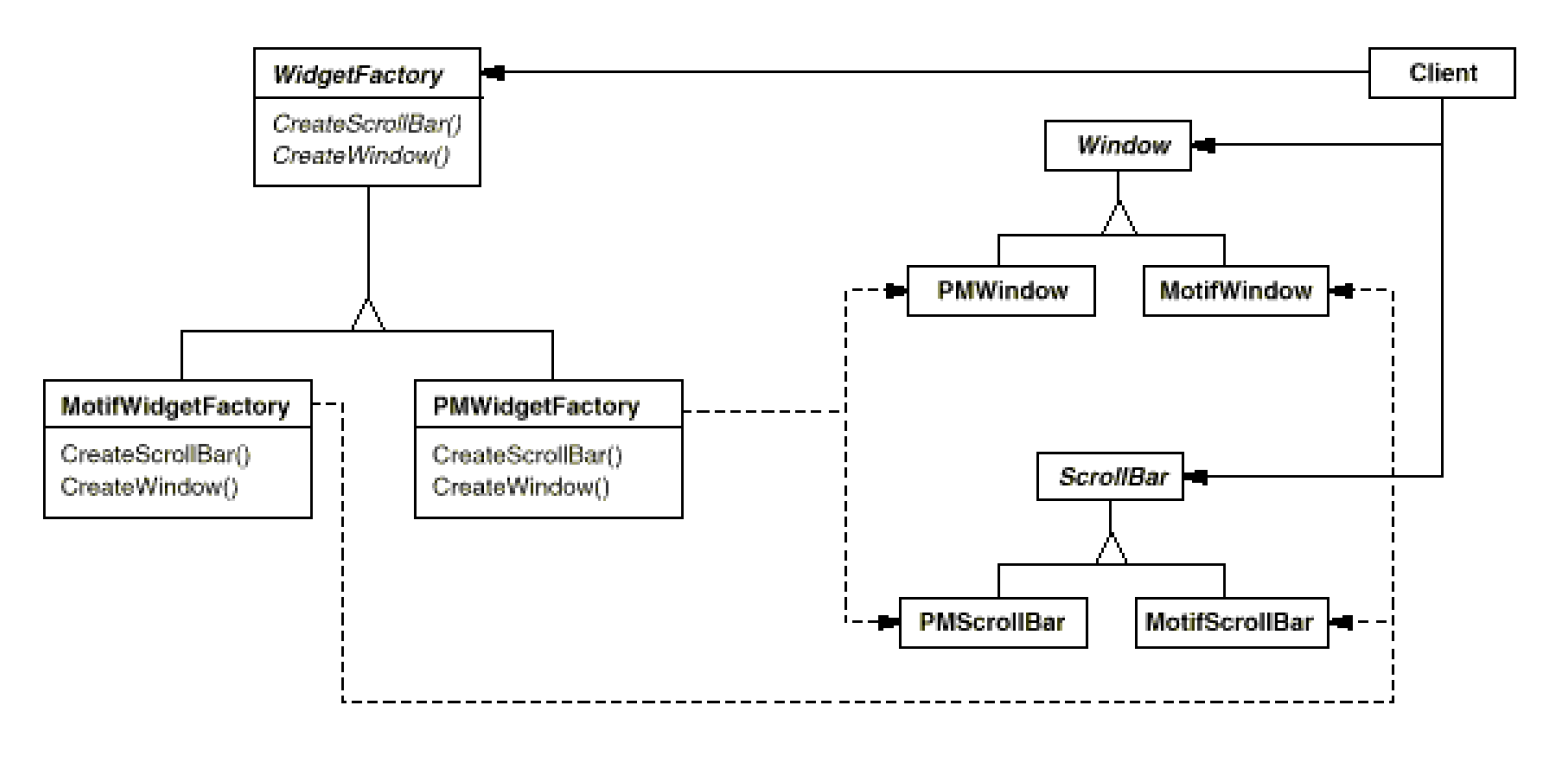
\includegraphics[scale=0.4]{motivation.png}
\end{center}
\end{frame}
%-------------------------------------------------------------------------------------------------

\subsection{Կիրառելիությունը}
%-------------------------------------------------------------------------------------------------
\begin{frame}\frametitle{Կիրառելիությունը}
Այս Ն.Ձ. պետք է օգտագործել երբ.
\vfill
{
    \scriptsize
    \begin{enumerate}
        \item Համակարգը պետք է անկախ լինի օբյեկտների ստեղծման և
        ներկայացման ձևից: \pause \vfill
        \item Անհրաժեշտ է խուսափել օբյեկտների հիերարխիային զուգահեռ Factory
        դասերի հիերարխիա կառուցելուց: \pause \vfill
        \item Երբ ստեղծվելիք օբյեկտի տիպը նշվում է ծրագրի կատարման
        ընթացքում (օրինակ ներբեռնելով) \pause \vfill
        \item Երբ օբյեկտը կարող է ունենալ քիչ քանակով իրարից տարբեր ներքին
        վիճակներ երբեմն ավելի նպատակահարմար է նախօրոք ստեղծել բոլոր իրարից
        տարբեր օբյեկտները և անհրաժեշտության դեպքում դրանք պատճենել նոր օբյեկտ
        ստեղծելու փոխարեն:
    \end{enumerate}
}
\end{frame}
%-------------------------------------------------------------------------------------------------

\section{Կառուցվածքը}
%-------------------------------------------------------------------------------------------------
\begin{frame}\frametitle{Կառուցվածքը}
\begin{center}
    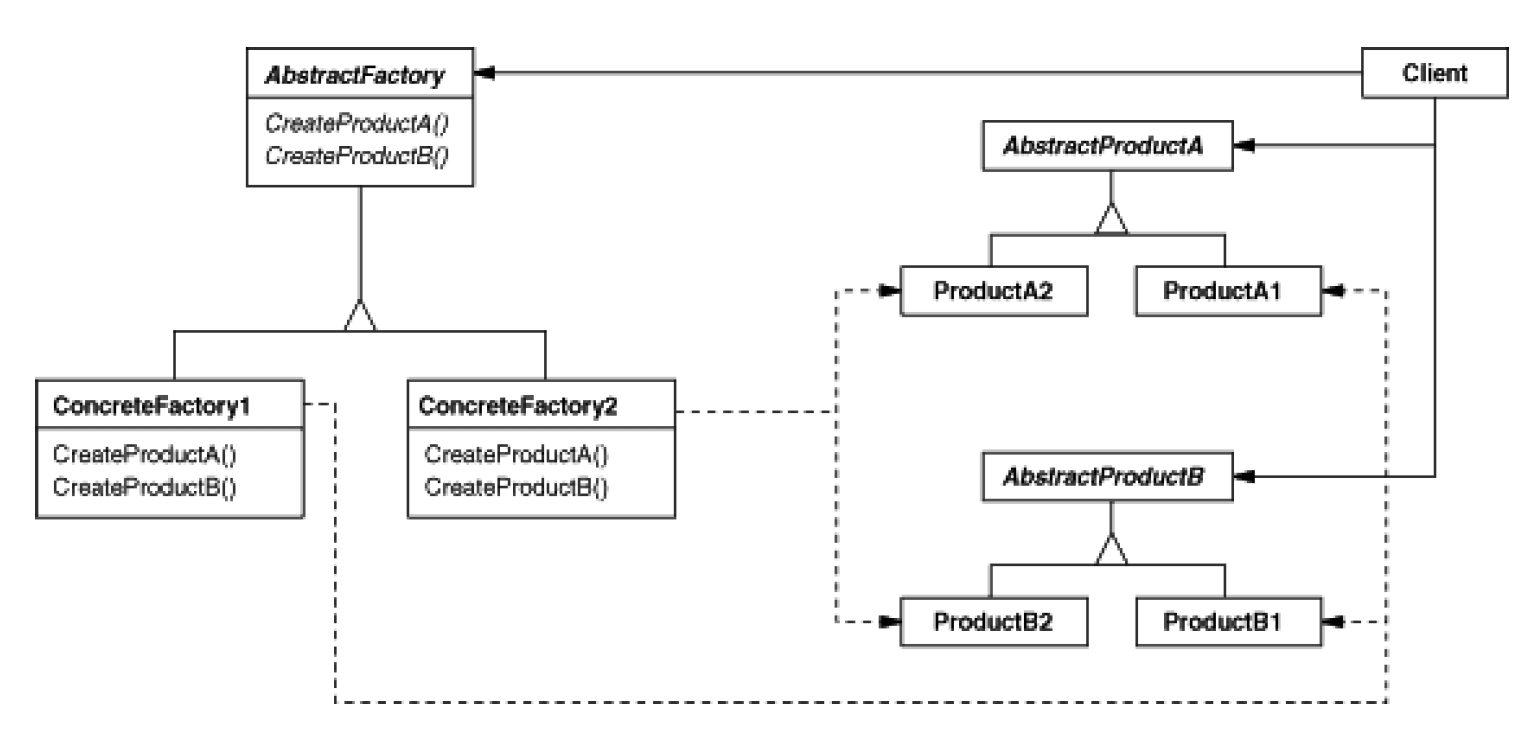
\includegraphics[scale=0.4]{structure.png}
\end{center}
\end{frame}
%-------------------------------------------------------------------------------------------------

\subsection{Հետևանքները}
%-------------------------------------------------------------------------------------------------
\begin{frame}\frametitle{Հետևանքները}
Այս Ն.Ձ. ունի հետևյալ առավելություններն ու թերությունները.
\vfill
\begin{enumerate}
    \item Առանձնացնում է կոնկրետ դասերը: \pause \vfill
    \item Ստեղծել նոր օբյեկտներ փոփոխելով արժեքները: \pause \vfill
    \item Ստեղծել նոր օբյեկտներ փոփոխելով կառուցվածքը: \pause \vfill
    \item Նվազեցնել ենթադասերի քանակը: \pause \vfill
    \item Դինամիկ կերպով կոնֆիգուրացնել կիրառությունը:
\end{enumerate}
\end{frame}
%-------------------------------------------------------------------------------------------------

\section{Իրականացումը}
%-------------------------------------------------------------------------------------------------
\begin{frame}\frametitle{Իրականացումը}
\begin{enumerate}
    \item Օգտագործելով prototype manager: \pause \vfill
    \item Clone գործողության իրականացումը: \pause \vfill
    \item Պատճենների ինիցիալիզացիան:
\end{enumerate}
\end{frame}
%-------------------------------------------------------------------------------------------------

\subsection{Օրինակ}
%-------------------------------------------------------------------------------------------------
\begin{frame}[fragile]\frametitle{Օրինակ}
\begin{english}
\begin{minted}{cpp}
class MazePrototypeFactory : public MazeFactory {

public:
    MazePrototypeFactory(Maze*, Wall*, Room*, Door*);

    virtual Maze* MakeMaze() const;

    virtual Room* MakeRoom(int) const;

    virtual Wall* MakeWall() const;

    virtual Door* MakeDoor(Room*, Room*) const;

private:
    Maze* prototypeMaze; Room* prototypeRoom;
    Wall* prototypeWall; Door* prototypeDoor;
};
\end{minted}
\end{english}
\end{frame}
%-------------------------------------------------------------------------------------------------

%-------------------------------------------------------------------------------------------------
\begin{frame}[fragile]\frametitle{Օրինակ}
\begin{english}
\begin{minted}{cpp}
MazePrototypeFactory::MazePrototypeFactory(Maze* m, Wall* w,
                                           Room* r, Door* d) {
    prototypeMaze = m; prototypeWall = w;
    prototypeRoom = r; prototypeDoor = d;
}

Wall* MazePrototypeFactory::MakeWall() const {

    return prototypeWall->Clone();
}

Door* MazePrototypeFactory::MakeDoor(Room* r1, Room *r2) const {

    Door* door = prototypeDoor->Clone();
    door->Initialize(r1, r2);
    return door;
}
\end{minted}
\end{english}
\end{frame}
%-------------------------------------------------------------------------------------------------

%-------------------------------------------------------------------------------------------------
\begin{frame}[fragile]\frametitle{Օրինակ}
\begin{english}
\begin{minted}[fontsize=\scriptsize]{cpp}
MazeGame game;
MazePrototypeFactory simpleMazeFactory(new Maze, new Wall,
                                       new Room, new Door);

Maze* maze = game.CreateMaze(simpleMazeFactory);


MazeGame game;
MazePrototypeFactory bombedMazeFactory(new Maze, new BombedWall,
                                       new RoomWithABomb, new Door);

Maze* maze = game.CreateMaze(bombedMazeFactor);
\end{minted}
\end{english}
\end{frame}
%-------------------------------------------------------------------------------------------------

%-------------------------------------------------------------------------------------------------
\begin{frame}[fragile]\frametitle{Օրինակ}
\begin{english}
\begin{minted}[fontsize=\scriptsize]{cpp}
class Door : public MapSite {

public:
    Door();

    Door(const Door& other) ) {
        room1 = other.room1; room2 = other.room2;
    }

    virtual void Initialize(Room* r1, Room* r2) ) {
        room1 = r1; room2 = r2;
    }

    virtual Door* Clone() const { return new Door(*this);}

    virtual void Enter();

private:
    Room* room1; Room* room2;
};
\end{minted}
\end{english}
\end{frame}
%-------------------------------------------------------------------------------------------------

\section{Առնչվող Ձևանմուշները}
%-------------------------------------------------------------------------------------------------
\begin{frame}\frametitle{Առնչվող Նախագծման Ձևանմուշները}
\begin{itemize}
    \item Abstract Factory \vfill
    \item Composite \vfill
    \item Decorator
\end{itemize}
\end{frame}
%-------------------------------------------------------------------------------------------------

\end{document}
